% !TEX root = ./main.tex

\chapter{关键模块与平台实现}

第三章从需求和总体架构层面对平台进行了设计，明确了前端展示层、后端代理层、模型推理与外部能力层之间的职责边界。本章按照当前平台的实际业务顺序展开：先说明平台入口与内容生成能力，再说明检测、审核、内容管理和部署实现。这样的组织方式能够对应“生成样本—保存入库—一键送检—检测分析—结果回看”的主流程，也避免把系统实现写成零散接口调用记录。

\section{平台入口与功能组织}

平台前端采用React、TypeScript、Vite和Ant Design实现，围绕首页、Deepfake生成、通用生成、虚假检测、不安全检测和内容管理六个页面组织功能。首页主要承担功能入口和任务分流作用，用户可从统一导航进入生成、检测、审核或内容管理流程。图~\ref{fig:platform-home} 展示了平台首页与整体功能入口。

\begin{figure}[H]
\centering
\includegraphics[width=0.98\textwidth]{figures/system/platform-home-white.png}
\caption{平台首页与整体功能模块}
\label{fig:platform-home}
\end{figure}

从页面组织角度看，平台将生成与检测拆分为独立页面，但在数据结构上保持联动。生成模块用于构造图像、视频和Deepfake样本；检测模块用于判断真实性与内容安全风险；内容管理模块用于保存生成样本、追踪检测记录、回看样本状态并支持再次送检。这种结构使平台既能用于系统演示，也能用于论文中的样本构建和功能验证。

\section{多源能力接入与标准化}

\subsection{统一能力组织思路}

本文平台接入的能力来源并不统一。一部分能力来自本地复现模型，例如UniversalFakeDetect、Stable Diffusion和ModelScope Text-to-Video；另一部分能力来自外部平台接口，例如火山引擎视觉智能接口和方舟多模态理解接口。若前端直接面向这些异构能力，将会面临参数格式不一致、鉴权方式不同、返回结构差异较大和异步机制复杂等问题。因此，系统实现中由后端代理层将多源能力封装为统一业务接口，再由前端按任务类型调用。

这一思路在代码层面主要体现为检测类接口和生成类接口两大类。检测类接口包括图像AI生成检测、视频AI生成检测、图像安全审核、视频安全审核以及本地图像伪造检测；生成类接口包括人脸替换、人脸动画、属性编辑、文生图、本地文生图、文生视频、本地文生视频和图生视频等。前端不直接感知某个任务究竟来自本地模型还是外部平台，而只需要按照业务类型提交请求。

\subsection{输入参数与结果结构标准化}

多源能力统一接入的关键是输入和输出标准化。对于输入层，图像任务统一接收 \texttt{imageUrl} 或 \texttt{imageBase64}；视频任务统一接收 \texttt{videoUrl} 或 \texttt{videoBase64}。系统还为视频理解任务补充了抽帧频率字段 \texttt{fps}，用于在0.2到5fps之间控制视频理解采样密度。后端会把视频URL或Base64统一封装为 \texttt{video\_url} 内容块，并在字段合法时附加fps参数。

在输出层，不同能力原生返回结构差异较大。本地检测模型更倾向于返回分数、阈值和模型信息；多模态理解接口则可能返回自然语言或嵌套JSON。为避免前端为每种能力单独编写渲染逻辑，后端对结果进行结构提取和字段映射。虚假检测统一关注真假结论、置信度、模型名称、原因说明和辅助展示信息；安全审核统一关注安全与否、处置建议、风险标签和说明文本。

多源检测结果的标准化流程如图~\ref{fig:result-normalize-flow} 所示。该流程体现了本文平台实现中的核心原则：前端只面向统一业务语义，后端负责吸收不同模型和接口之间的格式差异。

\begin{figure}[H]
\centering
\resizebox{0.96\textwidth}{!}{%
\begin{tikzpicture}[
  font=\small,
  node distance=9mm and 10mm,
  stdstep/.style={draw, rounded corners=3pt, thick, align=center, minimum width=2.7cm, minimum height=0.9cm, fill=blue!6},
  capbox/.style={draw, rounded corners=3pt, thick, align=center, minimum width=2.9cm, minimum height=0.9cm, fill=orange!10},
  normbox/.style={draw, rounded corners=3pt, thick, align=center, minimum width=2.9cm, minimum height=0.9cm, fill=green!8},
  arrow/.style={-Latex, thick}
]
  \node[stdstep] (input) {图像/视频输入\\URL或Base64};
  \node[stdstep, right=of input] (validate) {参数校验\\媒体类型识别};
  \node[stdstep, right=of validate] (route) {任务路由\\检测/审核/生成};
  \node[capbox, above right=7mm and 10mm of route] (local) {本地模型\\UFD/SD/T2V};
  \node[capbox, below right=7mm and 10mm of route] (external) {外部接口\\方舟/视觉智能};
  \node[normbox, right=4.0cm of route] (parse) {响应解析\\JSON提取/容错};
  \node[normbox, right=of parse] (map) {字段映射\\统一结果结构};
  \node[stdstep, right=of map] (ui) {前端渲染\\标签/分数/说明};

  \draw[arrow] (input) -- (validate);
  \draw[arrow] (validate) -- (route);
  \draw[arrow] (route) -- (local);
  \draw[arrow] (route) -- (external);
  \draw[arrow] (local.east) -| (parse.north);
  \draw[arrow] (external.east) -| (parse.south);
  \draw[arrow] (parse) -- (map);
  \draw[arrow] (map) -- (ui);
\end{tikzpicture}}
\caption{多源检测结果标准化处理流程}
\label{fig:result-normalize-flow}
\end{figure}


\section{内容生成模块实现}

\subsection{Deepfake生成能力实现}

Deepfake生成页主要覆盖人脸替换、人脸动画和属性编辑三类任务。人脸替换任务采用双图输入，源人脸图负责提供身份特征，目标模板图负责提供场景和姿态；后端根据具体模型版本将图片转换为外部接口所需的Base64字段，并完成签名鉴权、参数映射和结果提取。属性编辑任务则以原始人脸图和文本编辑指令为输入，用于验证“图像内容 + 文本指令”的联合编辑能力。人脸动画任务以首帧人脸图和动作描述为输入，输出短视频结果，主要服务于数字人驱动和伪造样本构造。

该模块的实现重点不是单纯生成效果展示，而是把Deepfake相关生成能力纳入统一平台。后端代理层屏蔽不同外部接口的鉴权方式和返回格式，前端只需要围绕源图、目标图、提示词和结果预览构建交互。图~\ref{fig:deepfake-generation} 展示了Deepfake生成页的实际运行界面，用于说明人脸替换、属性编辑或人脸动画能力在平台中的交互组织方式。

\begin{figure}[H]
\centering
\includegraphics[width=0.98\textwidth]{figures/system/deepfake.png}
\caption{Deepfake生成模块界面}
\label{fig:deepfake-generation}
\end{figure}

\subsection{通用图像与视频生成实现}

通用生成页覆盖文生图、文生视频和图生视频三类任务。文生图既支持外部图像生成接口，也保留本地Stable Diffusion服务作为开源模型入口；文生视频既支持外部Seedance系列模型，也支持本地ModelScope Text-to-Video服务；图生视频则支持参考图驱动、首帧驱动和首尾帧控制三种模式。这样处理的目的，是让平台能够覆盖图像生成、视频生成和跨模态生成三类样本来源。

结合当前实现，通用生成模块的重点增强主要体现在三方面。第一，图像生成模型扩展为Seedream 5.0、Seedream 4.5和本地Stable Diffusion，后端通过模型映射表选择实际接入点。第二，文生视频和图生视频扩展为Seedance 1.5 Pro、Seedance 2.0 Fast和Lite等不同能力，支持分辨率、比例、时长、随机种子、音频和水印等参数。第三，图生视频上传组件由单图上传扩展为多图槽位上传，可按顺序读取参考图，并根据模式映射为 \texttt{reference\_image}、\texttt{first\_frame} 和 \texttt{last\_frame} 等角色字段。

图~\ref{fig:text-to-image-result} 展示了平台文生图模块的运行界面。该截图对应“输入提示词—选择生成模型—返回媒体结果”的典型流程，用于说明生成能力已经通过前后端链路封装为可交互功能。

\begin{figure}[H]
\centering
\includegraphics[width=0.98\textwidth]{figures/system/text-to-image-result-white.png}
\caption{文生图生成结果展示界面}
\label{fig:text-to-image-result}
\end{figure}

为了让生成结果能够直接进入后续实验流程，当前平台在生成结果卡片中统一提供下载、保存到内容管理、重新生成和一键送检入口。生成结果出现后，前端首先根据任务类型提取图像或视频地址，再保存生成模型、提示词、来源模块和媒体类型等信息；当用户选择“一键送到检测模块”时，系统会在未保存样本的情况下先自动入库，并把样本编号随路由状态传递给检测页。这样实现后，文生图、文生视频、图生视频和Deepfake生成结果都可以复用同一套样本入库与送检逻辑，而不需要在每个生成页面重复编写检测输入转换代码。

\section{虚假内容检测模块实现}

\subsection{图像虚假检测实现}

图像虚假检测模块采用“双后端”方案。一类后端是本地部署的UniversalFakeDetect模型，用作可控、可复现的研究基线；另一类后端是外部多模态视觉理解接口，用于开放场景下的AI生成图像鉴别。前端页面提供检测模型选择，后端根据选择结果调用本地模型服务或外部接口，并统一返回 \texttt{isFake}、\texttt{confidence}、\texttt{model} 和 \texttt{details} 等字段。

本地模型服务通过Python接口封装后运行在独立端口，对外提供HTTP推理接口。Node.js后端负责把前端提交的URL或Base64图像转发给本地服务，并将模型返回的分数、阈值和说明映射为平台字段。外部图像鉴别接口则由后端把输入图像和固定判定提示词组织为视觉消息体，要求模型返回包含真假字段、置信度和原因说明的结构化JSON。

图~\ref{fig:fake-detect-page} 展示了虚假内容检测页的输入区和结果区组织方式。该页面在当前实现中已经从早期的标签页输入改为更紧凑的分段控制、上传预览、模型说明卡片和结果卡片布局，能够更清楚地表达“输入—选择模型—开始检测—查看结果”的流程。

\begin{figure}[H]
\centering
\includegraphics[width=0.98\textwidth]{figures/system/fake-detect-page-white.png}
\caption{虚假内容检测模块界面}
\label{fig:fake-detect-page}
\end{figure}

\subsection{视频虚假检测实现}

视频真假检测主要通过多模态视频理解接口实现。前端支持视频URL和本地视频上传两种输入方式，本地文件会被转换为Base64后提交给后端。后端将视频封装为统一的 \texttt{video\_url} 内容块，并结合固定的视频真假判定提示词调用视觉理解模型。相比图像任务，视频任务还需要考虑输入体积、抽帧频率和结果不确定性，因此前端提供fps参数控制，并在结果区展示置信度和原因说明。

当前版本尚未把本地视频伪造检测模型作为主链路接入，这与视频模型部署成本、显存占用和标注数据不足有关。但平台已经在输入结构、后端路由和结果展示上预留了位置，后续若接入D3类时序检测方法或其他本地视频模型，可按与图像检测相同的代理方式扩展。

\section{不安全内容审核模块实现}

\subsection{图像与视频审核链路实现}

不安全内容审核模块关注内容是否涉及暴力、色情、仇恨、赌博、敏感符号或其他违规风险。图像审核和视频审核均通过多模态视觉理解能力实现，区别主要在输入内容块和提示词约束。后端要求模型输出 \texttt{safe}、\texttt{suggestion}、\texttt{labels} 和 \texttt{reason} 等结构化字段，再将其映射为前端可展示的风险等级、标签和说明。

安全审核页在实现上进行了简化和强化：页面不再暴露多个未实际接入的模型下拉选择，而是明确展示“方舟视觉安全审核”这一固定链路，减少配置项对用户的误导；图像和视频输入组件统一采用上传/URL分段控制、预览区、操作按钮和模型说明卡片；视频安全审核同样支持fps参数。图~\ref{fig:unsafe-detect-page} 展示了不安全内容检测页的实际结果界面。

\begin{figure}[H]
\centering
\includegraphics[width=0.98\textwidth]{figures/system/unsafe-detect-page.png}
\caption{不安全内容审核模块界面}
\label{fig:unsafe-detect-page}
\end{figure}

\subsection{风险等级映射实现}

为了使图像审核和视频审核结果在页面上保持一致，系统将外部接口中的审核建议字段映射为平台风险等级：\texttt{pass} 对应低风险，\texttt{review} 对应中风险，\texttt{block} 对应高风险；同时将风险标签字段映射为前端标签。表~\ref{tab:risk-mapping} 给出了当前平台采用的风险映射方式。

\begin{table}[H]
\centering
\caption{安全审核结果风险映射}
\label{tab:risk-mapping}
\renewcommand{\arraystretch}{1.35}
\zihao{5}\songti
\begin{tabular}{C{2.2cm}C{3.0cm}L{8.5cm}}
\toprule
\textbf{接口建议} &
\textbf{平台风险等级} &
\multicolumn{1}{C{8.5cm}}{\textbf{页面展示与处理含义}} \\
\midrule
\texttt{pass} & 低风险 & 未发现明显违规内容，页面展示为可通过状态，仍保留模型说明用于回溯。 \\
\texttt{review} & 中风险 & 存在不确定或边界风险，页面提示建议人工复审，并展示风险标签和原因。 \\
\texttt{block} & 高风险 & 存在较明确违规或危险信号，页面展示为高风险并建议阻断或重点核查。 \\
\bottomrule
\end{tabular}
\end{table}

\section{结果展示与内容管理模块实现}

平台在实现上并未将检测结果停留在接口返回层，而是进一步构建了统一的风险展示和内容管理方式。对于虚假内容检测，前端主要通过真假标签、置信度进度条、模型名称和原因说明展示分析结果；对于不安全内容审核，则通过风险等级、建议级别、风险标签和说明性文本呈现审核判断。检测完成后，前端会把结论、分数、标签、检测模型和原始结果写入检测记录接口。如果检测输入来自生成样本，则一并写入 \texttt{sampleId}，后端据此更新样本的检测状态和最近检测结果。

内容管理模块当前已经由早期“结果查看入口”完善为“样本与检测记录中心”。样本列表展示生成内容的缩略图、媒体类型、来源模块、检测状态、最近结论和创建时间，并提供查看详情、送到AI生成检测、送到敏感检测、下载和删除等操作；检测记录列表展示检测对象、检测结论、分数、来源、模型和时间，并支持查看原始结果与下载检测对象。图~\ref{fig:data-output-page} 展示了内容管理页面的当前界面。

\begin{figure}[H]
\centering
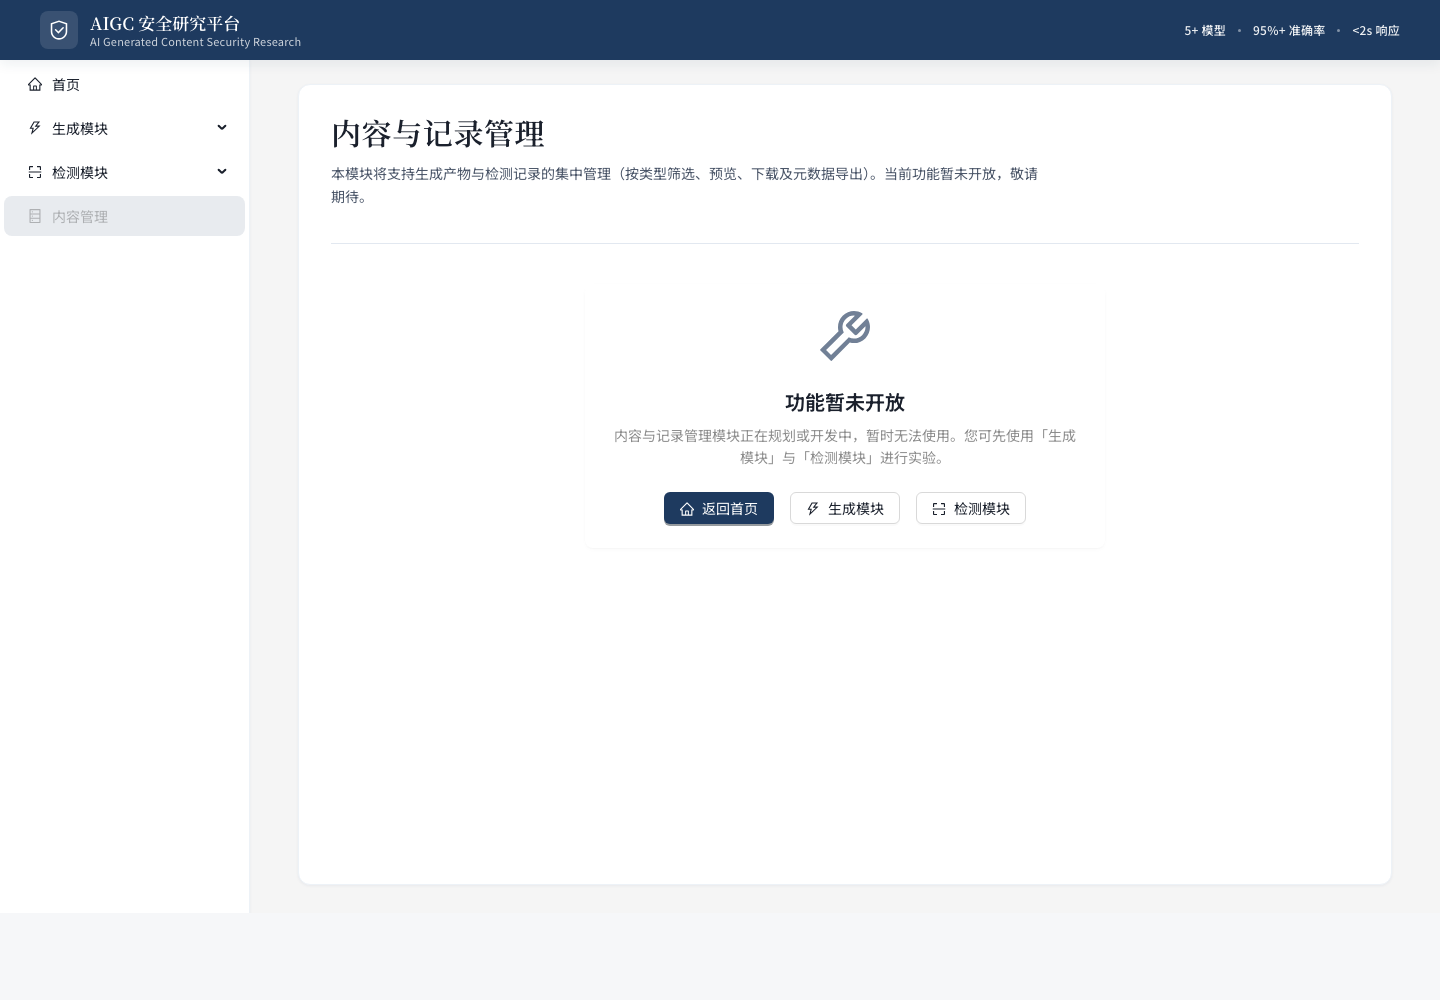
\includegraphics[width=0.98\textwidth]{figures/site-check/data-output.png}
\caption{样本与检测记录中心界面}
\label{fig:data-output-page}
\end{figure}

内容管理的后端实现由 \texttt{contentRoutes.cjs} 和 \texttt{contentStore.cjs} 共同完成，采用轻量JSON文件保存生成样本和检测记录，并把本地生成的Data URL媒体文件持久化到上传目录。该设计不追求复杂数据库能力，而是优先满足毕业设计阶段的可运行、可复核和易部署要求。表~\ref{tab:content-api-list} 给出了内容管理相关接口。

\begin{table}[H]
\centering
\caption{内容管理模块主要接口}
\label{tab:content-api-list}
\setlength{\tabcolsep}{3.5pt}
\renewcommand{\arraystretch}{1.35}
\zihao{5}\songti
\begin{tabular}{C{2.5cm}L{4.8cm}L{6.1cm}}
\toprule
\textbf{接口} &
\multicolumn{1}{C{4.8cm}}{\textbf{路径}} &
\multicolumn{1}{C{6.1cm}}{\textbf{功能说明}} \\
\midrule
保存样本 & \texttt{POST /api/data/save} & 保存生成图片或视频，写入媒体地址、来源模块、模型、提示词和检测状态。 \\
样本列表 & \texttt{GET /api/data/outputs} & 按时间倒序返回生成样本库，用于内容管理页展示和统计。 \\
样本详情 & \texttt{GET /api/data/outputs/:id} & 根据样本编号读取单个样本，用于详情回看和后续扩展。 \\
删除样本 & \texttt{DELETE /api/data/outputs/:id} & 从样本库移除样本；若已有关联检测记录，则保留记录中的来源快照。 \\
保存检测记录 & \texttt{POST /api/data/detections} & 保存检测结论、分数、标签、模型和原始结果，并更新关联样本检测状态。 \\
检测记录列表 & \texttt{GET /api/data/detections} & 返回全量检测历史，用于检测记录页展示和风险统计。 \\
样本检测历史 & \begin{tabular}[c]{@{}l@{}}\texttt{GET /api/data/outputs/}\\\texttt{:id/detections}\end{tabular} & 返回某个生成样本的关联检测记录，支持从样本详情查看历史。 \\
\bottomrule
\end{tabular}
\end{table}

一键送检的实现重点在于跨页面状态传递和媒体输入转换。生成页或内容管理页调用统一工具函数构造送检状态，其中包含目标检测类型、媒体类型、媒体地址、文件名、来源模块、模型名称和样本编号；检测页进入后读取该状态，并根据媒体地址类型选择URL输入或文件输入。对于本地持久化样本，前端会读取媒体文件并构造 \texttt{File} 对象，从而复用现有上传检测组件。检测完成后，记录接口将检测结果与样本编号关联，形成图~\ref{fig:one-click-detect-implementation} 所示的数据闭环。

\begin{figure}[H]
\centering
\resizebox{0.98\textwidth}{!}{%
\begin{tikzpicture}[
  font=\small,
  node distance=8mm and 9mm,
  implstep/.style={draw, rounded corners=3pt, thick, align=center, minimum width=2.8cm, minimum height=0.9cm, fill=blue!6},
  storestep/.style={draw, rounded corners=3pt, thick, align=center, minimum width=2.9cm, minimum height=0.9cm, fill=green!8},
  arrow/.style={-Latex, thick}
]
  \node[implstep] (result) {生成结果卡片\\图片/视频URL};
  \node[storestep, right=of result] (save) {保存样本\\获得sampleId};
  \node[implstep, right=of save] (transfer) {构造送检状态\\target/media/url};
  \node[implstep, right=of transfer] (page) {检测页接收\\自动填充输入};
  \node[implstep, below=1.0cm of page] (detect) {调用检测接口\\返回结构化结果};
  \node[storestep, left=of detect] (record) {保存检测记录\\关联sampleId};
  \node[storestep, left=of record] (status) {更新样本状态\\fake/unsafe};
  \node[implstep, left=of status] (center) {内容管理中心\\样本与历史回看};

  \draw[arrow] (result) -- (save);
  \draw[arrow] (save) -- (transfer);
  \draw[arrow] (transfer) -- (page);
  \draw[arrow] (page) -- (detect);
  \draw[arrow] (detect) -- (record);
  \draw[arrow] (record) -- (status);
  \draw[arrow] (status) -- (center);
  \draw[arrow] (center.north) .. controls +(0,1.0) and +(0,-1.0) .. (transfer.south);
\end{tikzpicture}}
\caption{一键送检与检测记录关联实现流程}
\label{fig:one-click-detect-implementation}
\end{figure}

\section{前后端平台开发与部署实现}

\subsection{前端页面职责}

当前前端页面与核心职责的对应关系如表~\ref{tab:frontend-pages} 所示。该表反映出本文平台并非单页接口演示，而是围绕生成、检测、审核和结果管理形成了相对完整的功能分区。

\begin{table}[H]
\centering
\caption{前端页面模块与职责}
\label{tab:frontend-pages}
\renewcommand{\arraystretch}{1.35}
\zihao{5}\songti
\begin{tabular}{C{2.9cm}L{4.3cm}L{6.8cm}}
\toprule
\textbf{页面模块} &
\multicolumn{1}{C{4.3cm}}{\textbf{主要输入}} &
\multicolumn{1}{C{6.8cm}}{\textbf{核心职责}} \\
\midrule
首页与导航页 & 无或少量演示入口 & 展示平台功能分区，引导用户进入生成、检测和内容管理流程。 \\
Deepfake生成页 & 源人脸、目标图像、驱动描述或编辑指令 & 支持人脸替换、人脸动画和属性编辑等典型深度伪造生成任务，并将结果保存或送检。 \\
通用生成页 & 文本提示词、参考图像和生成参数 & 支持文生图、文生视频、图生视频以及本地生成服务调用，提供生成结果入库与一键送检入口。 \\
虚假检测页 & 图像/视频文件或URL & 提供本地模型与外部接口两类真假检测入口，并展示置信度和原因说明。 \\
不安全检测页 & 图像/视频文件或URL & 对内容进行安全审核，输出风险等级、风险标签和处置建议。 \\
内容管理页 & 生成样本和检测记录 & 管理生成样本、检测历史、关联状态、下载、删除和再次送检。 \\
\bottomrule
\end{tabular}
\end{table}

\subsection{后端代理与任务调度}

后端服务基于Node.js和Express实现，是整个平台的能力汇聚中心。它主要承担五类职责：一是统一接收前端请求并按任务路由至不同能力；二是处理外部接口鉴权，包括Bearer Token和HMAC-SHA256签名两种主要模式；三是对多模态大模型返回结果进行结构提取与统一封装；四是对异步生成任务执行轮询调度，使前端能够以相对简洁的业务调用获得最终结果；五是维护生成样本库和检测记录库，使平台输出能够跨页面保留和追踪。

其中，异步任务封装和内容记录维护是后端实现中的两个关键点。以视频生成和图生视频为例，外部平台通常采用“提交任务—轮询查询—返回结果”的模式。如果前端直接处理这些步骤，将显著增加页面逻辑复杂度。后端通过统一封装轮询逻辑，将复杂异步流程收敛为单一业务接口。对于内容记录，后端则负责Data URL媒体持久化、JSON集合读写、损坏文件容错、检测状态更新和删除样本时的记录保留，从而保证内容管理页看到的是可复核的历史数据，而不是页面内存中的临时状态。

后端代理层对同步检测任务和异步生成任务的处理流程如图~\ref{fig:backend-dispatch-flow} 所示。对于图像检测等同步任务，后端主要完成参数转换、接口调用和结果归一化；对于视频生成等异步任务，后端还需要承担任务创建、轮询查询和超时处理。

\begin{figure}[H]
\centering
\resizebox{0.98\textwidth}{!}{%
\begin{tikzpicture}[
  font=\small,
  node distance=8mm and 9mm,
  schedstep/.style={draw, rounded corners=3pt, thick, align=center, minimum width=2.7cm, minimum height=0.9cm, fill=blue!6},
  proc/.style={draw, rounded corners=3pt, thick, align=center, minimum width=3.0cm, minimum height=0.9cm, fill=green!8},
  ext/.style={draw, rounded corners=3pt, thick, align=center, minimum width=3.0cm, minimum height=0.9cm, fill=orange!10},
  arrow/.style={-Latex, thick},
  dashedarrow/.style={-Latex, thick, dashed}
]
  \node[schedstep] (front) {前端页面\\提交业务请求};
  \node[proc, right=of front] (proxy) {后端代理\\参数校验/鉴权};
  \node[proc, right=of proxy] (route) {任务路由\\同步或异步};
  \node[ext, above right=7mm and 9mm of route] (sync) {同步能力调用\\图像检测/安全审核};
  \node[ext, below right=7mm and 9mm of route] (async) {异步任务创建\\文生视频/图生视频};
  \node[proc, right=3.9cm of route] (poll) {状态查询\\轮询/超时控制};
  \node[proc, right=of poll] (norm) {结果归一化\\字段映射/容错};
  \node[schedstep, right=of norm] (view) {前端展示\\标签/进度/说明};

  \draw[arrow] (front) -- (proxy);
  \draw[arrow] (proxy) -- (route);
  \draw[arrow] (route) -- (sync);
  \draw[arrow] (route) -- (async);
  \draw[arrow] (sync.east) -| (norm.north);
  \draw[arrow] (async.east) -| (poll.south);
  \draw[arrow] (poll) -- (norm);
  \draw[arrow] (norm) -- (view);
  \draw[dashedarrow] (poll.south) .. controls +(0,-1.0) and +(0,-1.0) .. (async.south);
\end{tikzpicture}}
\caption{后端代理层任务调度与结果归一化流程}
\label{fig:backend-dispatch-flow}
\end{figure}

\subsection{模型服务部署实现}

本地模型服务采用独立进程方式运行，其中图像虚假检测、本地文生图和本地文生视频分别封装为独立服务，并通过不同端口提供推理接口。结合当前项目进展，这些服务与后端代理进程共同部署在实验室服务器中，由前端通过后端统一访问。平台整体采用前后端分离部署方式：前端构建后作为静态页面运行，后端代理与本地模型服务作为独立进程驻留运行。

这种部署方式的优点在于结构清晰、便于调试和扩展。本地模型服务可以按需单独重启和替换，后端代理则负责维持稳定对外接口。内容管理数据以JSON文件和本地媒体目录形式保存在后端服务侧，部署时无需额外数据库即可完成样本和检测记录持久化。由于前端、后端和模型服务之间的边界较为明确，系统运行中出现问题时也更容易定位。尽管当前系统仍然存在视频本地检测能力和大规模样本验证不足等问题，但整体部署方案已经能够支撑平台核心功能运行。

\section{本章小结}

本章围绕平台关键模块说明了具体实现方式。首先，将平台截图展示集中放到实现章节，依次说明首页入口、Deepfake生成、通用生成、虚假检测、不安全审核和内容管理页面。随后，结合当前系统实现，说明了多模型生成、图生视频多参考图、视频理解fps参数、检测结果标准化、安全审核风险映射、生成样本入库和一键送检等关键改动。

总体来看，本文系统的重点并不在某一个单独模型本身，而在于通过后端代理、统一输入输出和模块化前端，把多类生成、检测与审核能力组织为一个可运行的平台。该实现为第五章的功能验证和实验分析提供了工程基础。
